\documentclass[12pt]{amsart}

\usepackage{tikz}
\usepackage{bbm}
\usetikzlibrary{3d,arrows,calc,positioning,decorations.pathreplacing,matrix} %,arrows.meta}

\usepackage{calligra,mathrsfs}
\usepackage[all]{xy}
\usepackage{float, comment}
\usepackage{mathtools}
\usepackage{amsmath}
\usepackage{amsthm}
\usepackage{amssymb}
\usepackage{amsbsy}
\usepackage{amstext}
\usepackage{amsopn}
%\usepackage{mathrsfs} % allows \mathscr
\usepackage[mathscr]{eucal}
\usepackage{enumerate}
\usepackage{xcolor}
\usepackage{graphicx} % allows \includegraphics{}s
\usepackage{tikz-cd}
\usepackage{scalerel}
\usepackage{microtype} % improves formattings
\usepackage[margin=1in,marginparwidth=0.8in, marginparsep=0.1in]{geometry}
\renewcommand{\baselinestretch}{1.2} % changes page formatting
\usepackage[pagebackref, bookmarks=true, bookmarksopen=true, bookmarksdepth=3,bookmarksopenlevel=2, colorlinks=true, linkcolor=blue, citecolor=blue, filecolor=blue, menucolor=blue, urlcolor=blue]{hyperref}
% \usepackage{newtxtext} % improves font appearance
\usepackage{tikz}
\usepackage{bbm}
\usepackage[all]{xy}
\usetikzlibrary{arrows,calc,positioning,decorations.pathreplacing} %,arrows.meta}

%Path relative to the main .tex file 
\graphicspath{ {./figures/} }

\newcommand{\blue}{\color{blue}}
\newcommand{\red}{\color{red}}

\numberwithin{equation}{section}
\newtheorem{Theorem}[equation]{Theorem}
\newtheorem{Proof}[equation]{Proof}
\newtheorem{Proposition}[equation]{Proposition} 
\newtheorem{Lemma}[equation]{Lemma}
\newtheorem{Open}[equation]{Open Question}
\newtheorem{Corollary}[equation]{Corollary}
\newtheorem{Conjecture}[equation]{Conjecture}
\newtheorem{Specialthm}{Theorem}
\newtheorem{Question}{Question}

\theoremstyle{definition}
\newtheorem{Remark}[equation]{Remark}
\newtheorem{Example}[equation]{Example}
\newtheorem{Definition}[equation]{Definition}

\numberwithin{figure}{section}

\def\la{\langle}
\def\ra{\rangle}
\def\ttimes{\widetilde{\times}}
\def\tbox{\widetilde{\boxtimes}}
\def\bbox{{\boxtimes}}
\def\O{\mathcal{O}}
\def\K{\mathcal{K}}
\def\bG{\mathbb{G}}
\newcommand{\gr}{\mathrm{gr}}
\newcommand{\wt}{\text{wt}}
\newcommand{\mb}[1]{\mathbf{#1}}
\newcommand{\fsl}{\mathfrak{sl}}
\newcommand{\fg}{\mathfrak{g}}
\newcommand{\fn}{\mathfrak{n}}
\newcommand{\bk}{{\mathbbm k}}
\newcommand{\A}{\mathbb{A}}
\newcommand{\C}{\mathbb{C}}
\newcommand{\D}{\mathbb{D}}
\newcommand{\E}{\mathbb{E}}
\newcommand{\G}{\mathbb{G}}
\newcommand{\bN}{\mathbb{N}}
\renewcommand{\P}{\mathbb{P}}
\newcommand{\Q}{\mathbb{Q}}
\newcommand{\Z}{\mathbb{Z}}
\newcommand{\bfC}{{\mathbf{C}}}
\newcommand{\bfD}{{\mathbf{D}}}
\newcommand{\bfI}{{\mathbf{I}}}
\newcommand{\cA}{\mathcal{A}}
\newcommand{\cB}{\mathcal{B}}
\newcommand{\cC}{\mathcal{C}}
\newcommand{\cD}{\mathcal{D}}
\newcommand{\cE}{\mathcal{E}}
\newcommand{\cF}{\mathcal{F}}
\newcommand{\cG}{\mathcal{G}}
\newcommand{\cH}{\mathcal{H}}
\newcommand{\cK}{\mathcal{K}}
\newcommand{\cL}{\mathcal{L}}
\newcommand{\cM}{\mathcal{M}}
\newcommand{\cN}{\mathcal{N}}
\newcommand{\cO}{\mathcal{O}}
\newcommand{\cP}{\mathcal{P}}
\newcommand{\cQ}{\mathcal{Q}}
\newcommand{\cR}{\mathcal{R}}
\newcommand{\cS}{\mathcal{S}}
\newcommand{\cT}{\mathcal{T}}
\newcommand{\cU}{\mathcal{U}}
\newcommand{\cV}{\mathcal{V}}
\newcommand{\cW}{\mathcal{W}}
\newcommand{\cX}{\mathcal{X}}
\newcommand{\cY}{\mathcal{Y}}
\newcommand{\sW}{\mathscr{W}}
\newcommand{\sX}{\mathscr{X}}
\newcommand{\sY}{\mathscr{Y}}
\newcommand{\sZ}{\mathscr{Z}}

\newcommand{\hs}{\heartsuit}
\newcommand{\bul}{\bullet}
\newcommand{\ga}{\gamma}
\newcommand{\al}{\alpha}
\newcommand{\be}{\beta}

%Commands for Lecture 14
\newcommand{\on}[1]{\operatorname{#1}}
\newcommand{\cI}{\mathcal{I}}
\newcommand{\Gr}{\on{Gr}}
\newcommand{\TeL}{\on{TL}}
\newcommand{\Rcheck}{\breve{R}}
\newcommand{\Stil}{\tilde{S}}
\usepackage{tikzit}
\input{tikzit_styles.tikzstyles}

%% code from mathabx.sty and mathabx.dcl
\DeclareFontFamily{U}{mathx}{\hyphenchar\font45}
\DeclareFontShape{U}{mathx}{m}{n}{
	<5> <6> <7> <8> <9> <10>
	<10.95> <12> <14.4> <17.28> <20.74> <24.88>
	mathx10
}{}
\DeclareSymbolFont{mathx}{U}{mathx}{m}{n}
\DeclareFontSubstitution{U}{mathx}{m}{n}
\DeclareMathAccent{\widecheck}{0}{mathx}{"71}
\DeclareMathSymbol{\shortminus}{\mathbin}{AMSa}{"39}

\DeclareRobustCommand{\SkipTocEntry}[5]{}

\newcommand{\arrtip}{latex'}

\begin{document}
\title{Notes on Schubert Calculus and Quantum Integrability}

\begin{abstract}
\end{abstract}

\maketitle

\setcounter{tocdepth}{1}

\tableofcontents

\section{Introduction}

\thispagestyle{empty}

Here is a template for a simple commutative diagram in tikz:
\begin{equation*}
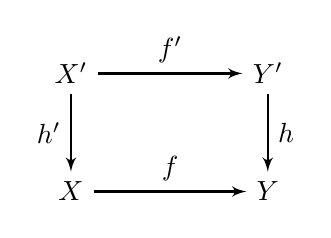
\begin{tikzpicture}
[baseline=(current  bounding  box.center),thick,>=\arrtip]
\node (a) at (0,0) {$X'$};
\node (b) at (2.5,0) {$Y'$};
\node (c) at (0,-1.5) {$X$};
\node (d) at (2.5,-1.5) {$Y$};
\draw[->] (a) to node[above] {$f' $} (b);
\draw[->] (b) to node[right] {$h $} (d);
\draw[->] (a) to node[left] {$h' $}(c);
\draw[->] (c) to node[above] {$f $} (d);
\end{tikzpicture}
\end{equation*}

Here is a template for an elaborate commutative diagram in tikz:
\begin{equation*}
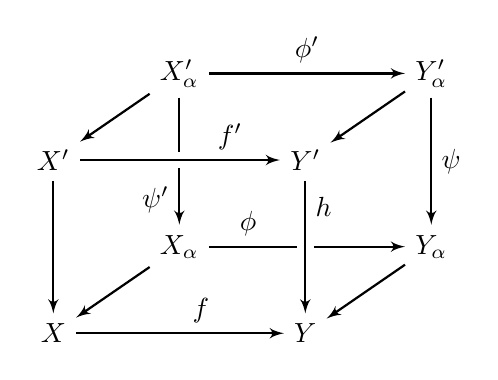
\begin{tikzpicture}[baseline=(current  bounding  box.center),thick,>=\arrtip]
\newcommand*{\ha}{1.6}; \newcommand*{\hb}{1.6}; \newcommand*{\hc}{1.6};
\newcommand*{\va}{-1.1}; \newcommand*{\vb}{-1.1}; \newcommand*{\vc}{-1.1};
\node (ab) at (\ha,0) {$X_\al'$};
\node (ad) at (\ha+\hb+\hc,0) {$Y_\al'$};
\node (ba) at (0,\va) {$X'$};
\node (bc) at (\ha+\hb,\va) {$Y'$};
\node (cb) at (\ha,\va+\vb) {$X_\al$};
\node (cd) at (\ha+\hb+\hc,\va+\vb) {$Y_\al$};
\node (da) at (0,\va+\vb+\vc) {$X$};
\node (dc) at (\ha+\hb,\va+\vb+\vc) {$Y$};
\draw[->] (ab) to node[above] {$\phi' $} (ad);
\draw[->] (ab) to node[above] {$ $} (ba);
\draw[->] (ab) to node[left,pos=.8] {$\psi' $} (cb);
\draw[->] (ad) to node[above] {$ $} (bc);
\draw[->] (ad) to node[right] {$\psi $} (cd);
\draw[->] (ba) to node[above] {$ $} (da);
\draw[->] (cb) to node[above,pos=.2] {$\phi $} (cd);
\draw[->] (cb) to node[above] {$ $} (da);
\draw[->] (cd) to node[above] {$ $} (dc);
\draw[->] (da) to node[above,pos=.6] {$f $} (dc);
\draw[-,line width=6pt,draw=white] (ba) to  (bc);
\draw[->] (ba) to node[above,pos=.75] {$f' $} (bc);
\draw[-,line width=6pt,draw=white] (bc) to  (dc);
\draw[->] (bc) to node[right,pos=.2] {$h $} (dc);
\end{tikzpicture}
\end{equation*}


\section{Lecture 1 (Allen Knutson)}

Let $V$ be a $k$-plane in $\C^n$ with basis represented as a $k\times n$ matrix with basis elements as row vectors. Put this matrix into Reduced Row Echelon Form and consider left action by $GL_k(\C)$ and right action by upper triangular matrices to get an open subgroup of \textit{right word row operations}.

\begin{Theorem}
	A matrix $\text{Mat}_n(\C)$ acted on the left by $GL_k(\C)$ downward row operations and  on the right by upper triangular matrices rightward column operations, that is,
	$$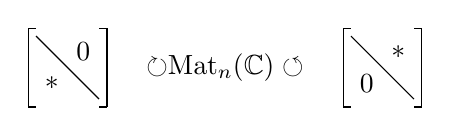
\begin{tikzpicture}
		\node (a) at (.3,.3) {$*$};
		\node (b) at (.7,.7) {$0$};
		\draw [-] (.9,.1) to (.1,.9);
		\draw[-] (0,0) to (0,1);
		\draw[-] (1,0) to (1,1);
		\draw[-] (0,0) to (.1,0);
		\draw[-] (0,1) to (.1,1);
		\draw[-] (.9,0) to (1,0);
		\draw[-] (.9,1) to (1,1);
		\node (c) at (2.5,.5) {$\circlearrowright$Mat$_n(\C)\circlearrowleft$};
		\node (a) at (4.3,.3) {$0$};
		\node (b) at (4.7,.7) {$*$};
		\draw [-] (4.9,.1) to (4.1,.9);
		\draw[-] (4,0) to (4,1);
		\draw[-] (5,0) to (5,1);
		\draw[-] (4,0) to (4.1,0);
		\draw[-] (4,1) to (4.1,1);
		\draw[-] (4.9,0) to (5,0);
		\draw[-] (4.9,1) to (5,1);
	\end{tikzpicture}$$
	has one orbit for each partial permutation matrix. This is the \textbf{Bruhet decomposition} of the matrix.
\end{Theorem}

\begin{Definition}
	A matrix \textbf{Schubert Variety} is $\overline{X_{\pi}}:=\overline{B_-\pi B_+}$ where $\pi$ is the permutation matrix.
\end{Definition}

\begin{Theorem}
	$\overline{X_\pi}$ is the set of $n\times n$ matrices, $M$, such that for all $i,j\in[n]$, the $i\times j$ submatrix of $M$ is less than or equal to the $i\times j$ submatrix of $\pi$. That is, the determinants summarized by these conditions generate a prime ideal whose vanishing set is $\overline{X_\pi}$.
\end{Theorem}

As an example, consider $\pi=3142$ pictured below:

\begin{center}
	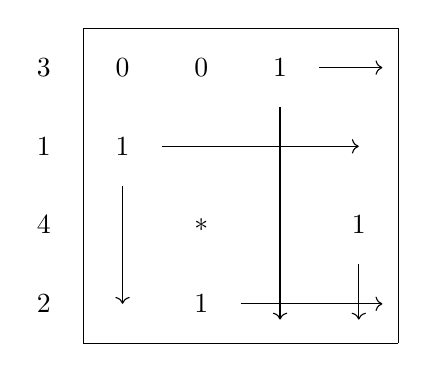
\begin{tikzpicture}
		\node (40) at (0,.5) {$2$};
		\node (30) at (0,1.5) {$4$};
		\node (20) at (0,2.5) {$1$};
		\node (10) at (0,3.5) {$3$};
		\node (21) at (1,2.5) {$1$};
		\node (11) at (1,3.5) {$0$};
		\node (42) at (2, .5) {$1$};
		\node (32) at (2,1.5) {$*$};
		\node (12) at (2,3.5) {$0$};
		\node (13) at (3,3.5) {$1$};
		\node (34) at (4,1.5) {$1$};
		\draw[-] (.5,0) to (.5,4);
		\draw[-] (4.5,0) to (4.5,4);
		\draw[-] (.5,0) to (4.5,0);
		\draw[-] (.5,4) to (4.5,4);
		\draw[->] (2.5,.5) to (4.3,.5);
		\draw[->] (1,2) to (1,.5);
		\draw[->] (1.5,2.5) to (4,2.5);
		\draw[->] (4,1) to (4,.3);
		\draw[->] (3,3) to (3,.3);
		\draw[->] (3.5,3.5) to (4.3,3.5);
	\end{tikzpicture}
\end{center}
The arrows are referred to as \textbf{death rays} since each leading one eliminates the entries to the right of and below it. In this example we have that $$m_{11}=m_{12}=0=\det\left ( \begin{array}{cc} m_{21} & m_{22} \\ m_{31} & m_{32}  \end{array}\right )$$ and the associated \textbf{Rothe diagram} is $$\left [ \begin{array}{cc} 0 & 0 \\ & *\end{array}\right ]$$

Two natural questions arise. First, how big is $\overline{X_\pi}$? We see that \begin{align*}
	\dim\overline{X_\pi}&=\dim(B_-\pi B_+) \\
	&= \dim(B_-\times B_+)-\dim(\text{stab}(\pi))\\
	&=\text{the number of entries crossed out in the death ray diagram}\\
	&=\dim T_\pi(B_-\pi B_+)\\
	&=\dim(b_-\pi+\pi b_+)
\end{align*}
Where $b_-$ and $b_+$ are lie algebras. Hence the codimension of $\overline{X_\pi}$ is the number of entries in the Rothe diagram.

\begin{Theorem}
	The only essential rank conditions are at the southeast corners of the Rothe diagram.
\end{Theorem}

The second question is what is the volumn of $\P(\overline{X_\pi})$?
Considering the degree as a projective variety, we get the following axioms for $Y\subseteq\P(V)$ defined by some homogeneous ideal.
\begin{enumerate}
	\item[(0)] The degree of $p^1$ is 1.
	\item If $Y$ is reducible, that is the ideal is not prime, such that $Y=Y_1\cup Y_2\cup\cdots\cup Y_k$ and $I\subseteq P_i$ is minimal, then the degree of $Y$ is the sum over the top dimensional components of the product of the multiplicity of $Y_i$ and the degree of $Y_i$.
	\item If $W\subseteq V$ is a hyperplane and $\P(W)\supseteq Y$ then the degree of $Y$ in $\P(V)$ is equal to the degree of $Y$ in $\P(W)$.
	\item If $W\subseteq V$ is a hyperplane and Y is reduced and irreducible, that is I is prime and $Y\subseteq \P(W)$, then the degree of $Y$ in $\P(V)$ is equal to the degree of $Y\cap\P(W)$ in $\P(W)$.
	
\end{enumerate}

What is the degree of $\P(\overline{X_\pi})$? Consider the base case where $$\pi=w_0^{(n)}=
\vcenter{\hbox{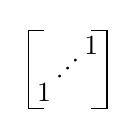
\begin{tikzpicture}
			\node at (.2,.2) {1};
			\node at (.8,.8) {1};
			\node at (.4,.4) {$\cdot$};
			\node at (.5,.5) {$\cdot$};
			\node at (.6,.6) {$\cdot$};
			\draw[-] (0,0) to (0,1);
			\draw[-] (0,0) to (.2,0);
			\draw[-] (0,1) to (.2,1);
			\draw[-] (1,0) to (1,1);
			\draw[-] (.8,0) to (1,0);
			\draw [-] (.8,1) to (1,1);
\end{tikzpicture}}}$$.

After eliminating entries via death rays we see that
$\overline{X_\pi}=\left \{ M: \vcenter{\hbox{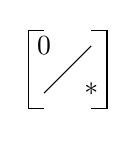
\begin{tikzpicture}
			\node at (.2,.8) {0};
			\node at (.8,.2) {*};
			\draw[-] (.2,.2) to (.8,.8);
			\draw[-] (0,0) to (0,1);
			\draw[-] (0,0) to (.2,0);
			\draw[-] (0,1) to (.2,1);
			\draw[-] (1,0) to (1,1);
			\draw[-] (.8,0) to (1,0);
			\draw [-] (.8,1) to (1,1);
\end{tikzpicture}}}\right \}$
where the $0$'s in the upper left of the matrix aligns with axiom 2 and the free variables in the lower left align with axiom 3. This gives us that $\deg(\overline{X_\pi})=1$.

If $\pi\neq w_0^{(n)}$ pick $i\in[n]$ least such that $\pi(i)\neq w_0^{(n)}(i)=n+1-i$. Then $W:=\{ M: m_i\pi(i)=0\}$ and $$\overline{X_\pi}\cap W=\overline{X_\pi}\cap\left\{ \vcenter{\hbox{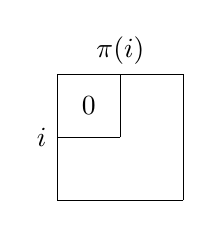
\begin{tikzpicture}
			\node at (0,0) {$i$};
			\node at (1,1.1) {$\pi(i)$};
			\node at (.6,.4) {$0$};
			\draw[-] (.2,.8) to (.2,-.8);
			\draw[-] (.2,-.8) to (1.8,-.8);
			\draw[-] (1.8,-.8) to (1.8,.8);
			\draw[-] (1.8,.8)to (.2,.8);
			\draw[-] (1,0) to (1,.8);
			\draw[-] (.2,0) to (1,0);
\end{tikzpicture}}}\right\}\circlearrowleft B_-\times B_+ \text{ invariant}$$ which is the union of $\overline{X_{\pi'}}$ over certain $\pi'$ none of which are strictly partial permutations and all multiplicities are $1$.

\begin{Definition}
	A \textbf{pipe dream} for $\pi$ is a diagram $$\vcenter{\hbox{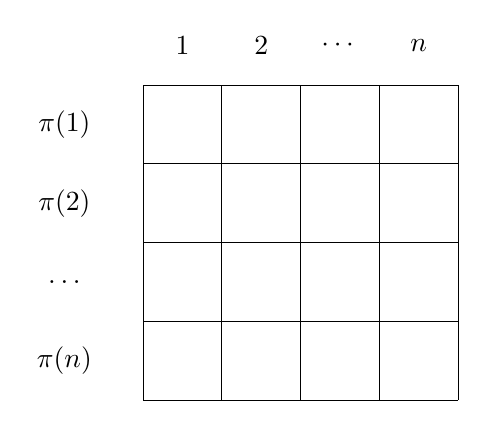
\begin{tikzpicture}
				\draw[-] (1,4) to (5,4);
				\draw[-] (5,4) to (5,0);
				\draw[-] (5,0) to (1,0);
				\draw[-] (1,0) to (1,4);
				\node (1) at (1.5,4.5) {$1$};
				\node (2) at (2.5,4.5) {$2$};
				\node (...) at (3.5,4.5) {$\cdots$};
				\node (n) at (4.5,4.5) {$n$};
				\node (p1) at (0,3.5) {$\pi(1)$};
				\node (p2) at (0,2.5) {$\pi(2)$};
				\node (p) at (0,1.5) {$\hdots$};
				\node (pn) at (0,.5) {$\pi(n)$};
				\draw[-] (2,4) to (2,0);
				\draw[-] (3,4) to (3,0);
				\draw[-] (4,4) to (4,0);
				\draw[-] (1,1) to (5,1);
				\draw[-] (1,2) to (5,2);
				\draw[-] (1,3) to (5,3);
				\draw[-] (1,4) to (5,4);
	\end{tikzpicture}}}$$
	where each box is filed in with one of two tiles: crosses $\vcenter{\hbox{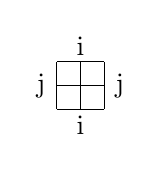
\begin{tikzpicture}
				\node at (0,.5) {j};
				\node at (.5,1) {i};
				\node at (1,.5) {j};
				\node at (.5,0) {i};
				\draw[-] (.2,.2) to (.2,.8);
				\draw[-] (.2,.8) to (.8,.8);
				\draw[-] (.8,.8) to (.8,.2);
				\draw[-] (.8,.2) to (.2,.2);
				\draw[-] (.2,.5) to (.8,.5);
				\draw[-] (.5,.2) to (.5,.8);
	\end{tikzpicture}}}$ when $i\leq j$ and elbows $\vcenter{\hbox{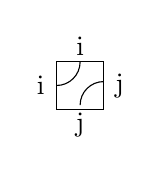
\begin{tikzpicture}
				\node at (0,.5) {i};
				\node at (.5,1) {i};
				\node at (1,.5) {j};
				\node at (.5,0) {j};
				\draw[-] (.2,.2) to (.2,.8);
				\draw[-] (.2,.8) to (.8,.8);
				\draw[-] (.8,.8) to (.8,.2);
				\draw[-] (.8,.2) to (.2,.2);
				\draw (.2,.5) arc[start angle=-90, end angle=0, radius=.3];
				\draw (.5,.25) arc[start angle=180, end angle=90, radius=.3];
	\end{tikzpicture}}}$ when $i\neq j$.
\end{Definition}

\begin{Theorem}
	The degree of $\overline{X_\pi}$ is the number of pipe dreams of $\pi$.
\end{Theorem}
For a torus $T\cong (\C^x)^N$ and $Y\subseteq V)\circlearrowleft T$ where $Y$ is a $T$-invariant subvariety and $V$ is a $T$-representation can soup up the degree to a $T$-equivariant cohomology class. 

Our above axioms hold from above with the exception of axiom 2 which can be rewritten at follows: \begin{enumerate}
	\item[(2)] $[Y\subseteq V]$ equals the weight of $T(V/W)[Y\subseteq W]$ for $T\in T^*$. The $T^*$ weight lattice is given by Hom$(T,\C^x)\cong\Z^N$ such that for $\Lambda=(\lambda_1,\ldots,\lambda_N)\in\Z^N$ and $t=(t_1,\ldots,t_N)\in(\C^x)^N$, $\Lambda\cdot t=\prod\limits_{i=1}^N t_i^{\lambda_i}$. Then $[Y\subseteq V]\in\text{Sum}(T^*)\cong\Z[Y_1,\ldots,Y_n]$.
\end{enumerate}

\begin{Definition}
	The \textbf{Double Schubert Polynomial} is $S_\pi(X,Y)=[\overline{X_\pi}\subseteq\text{Mat}_n]$ with respect to $T\times T\circlearrowright\text{Mat}_n$ such that $\overline{S_\pi}(X,Y)=\sum\limits_{\text{p}}\prod\limits_{\text{c}}(X_{\text{row}}-Y_{\text{col}})$ where $p$ stands for pipe dreams for $\pi$ and $c$ represents crosses. 
\end{Definition}
Consider the possible pipe dreams for $\pi=132$.
\begin{center}
	$\vcenter{\hbox{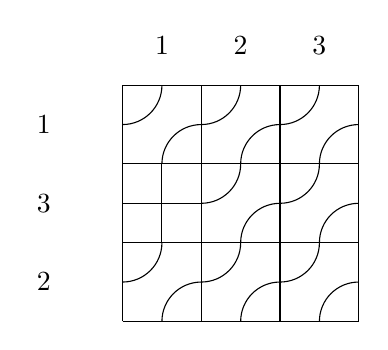
\begin{tikzpicture}
				\draw[-] (1,4) to (4,4);
				\draw[-] (4,4) to (4,1);
				\draw[-] (4,1) to (1,1);
				\draw[-] (1,1) to (1,4);
				\node (1) at (1.5,4.5) {$1$};
				\node (2) at (2.5,4.5) {$2$};
				\node (3) at (3.5,4.5) {$3$};
				\node (p1) at (0,3.5) {$1$};
				\node (p2) at (0,2.5) {$3$};
				\node (p3) at (0,1.5) {$2$};
				\draw[-] (2,4) to (2,1);
				\draw[-] (3,4) to (3,1);
				\draw[-] (4,4) to (4,1);
				\draw[-] (1,1) to (4,1);
				\draw[-] (1,2) to (4,2);
				\draw[-] (1,3) to (4,3);
				\draw[-] (1,4) to (4,4);
				\draw (1,3.5) arc[start angle=-90, end angle=0, radius=.5]; %11
				\draw (1.5,3) arc[start angle=180, end angle=90, radius=.5]; 
				\draw (2,3.5) arc[start angle=-90, end angle=0, radius=.5]; %12
				\draw (2.5,3) arc[start angle=180, end angle=90, radius=.5];
				\draw (3,3.5) arc[start angle=-90, end angle=0, radius=.5]; %13
				\draw (3.5,3) arc[start angle=180, end angle=90, radius=.5];
				\draw[-] (1,2.5) to (2,2.5); %21
				\draw[-] (1.5,3) to (1.5,2);
				\draw (2,2.5) arc[start angle=-90, end angle=0, radius=.5]; %22
				\draw (2.5,2) arc[start angle=180, end angle=90, radius=.5];
				\draw (3,2.5) arc[start angle=-90, end angle=0, radius=.5]; %23
				\draw (3.5,2) arc[start angle=180, end angle=90, radius=.5];
				\draw (1,1.5) arc[start angle=-90, end angle=0, radius=.5]; %31
				\draw (1.5,1) arc[start angle=180, end angle=90, radius=.5];
				\draw (3,1.5) arc[start angle=-90, end angle=0, radius=.5]; %32
				\draw (2.5,1) arc[start angle=180, end angle=90, radius=.5];
				\draw (2,1.5) arc[start angle=-90, end angle=0, radius=.5]; %33
				\draw (3.5,1) arc[start angle=180, end angle=90, radius=.5];
	\end{tikzpicture}}}$
	\hspace{10mm} and \hspace{10mm}
	$\vcenter{\hbox{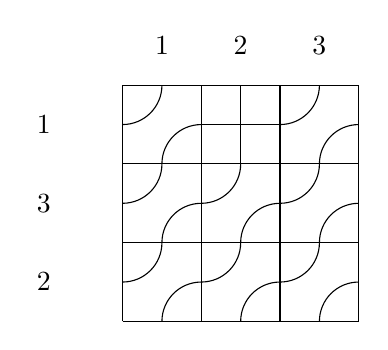
\begin{tikzpicture}
				\draw[-] (1,4) to (4,4);
				\draw[-] (4,4) to (4,1);
				\draw[-] (4,1) to (1,1);
				\draw[-] (1,1) to (1,4);
				\node (1) at (1.5,4.5) {$1$};
				\node (2) at (2.5,4.5) {$2$};
				\node (3) at (3.5,4.5) {$3$};
				\node (p1) at (0,3.5) {$1$};
				\node (p2) at (0,2.5) {$3$};
				\node (p3) at (0,1.5) {$2$};
				\draw[-] (2,4) to (2,1);
				\draw[-] (3,4) to (3,1);
				\draw[-] (4,4) to (4,1);
				\draw[-] (1,1) to (4,1);
				\draw[-] (1,2) to (4,2);
				\draw[-] (1,3) to (4,3);
				\draw[-] (1,4) to (4,4);
				\draw (1,3.5) arc[start angle=-90, end angle=0, radius=.5]; %11
				\draw (1.5,3) arc[start angle=180, end angle=90, radius=.5]; 
				\draw[-] (2.5,4) to (2.5,3); %12
				\draw[-] (2,3.5) to (3,3.5);
				\draw (3,3.5) arc[start angle=-90, end angle=0, radius=.5]; %13
				\draw (3.5,3) arc[start angle=180, end angle=90, radius=.5];
				\draw (1,2.5) arc[start angle=-90, end angle=0, radius=.5]; %21
				\draw (1.5,2) arc[start angle=180, end angle=90, radius=.5];
				\draw (2,2.5) arc[start angle=-90, end angle=0, radius=.5]; %22
				\draw (2.5,2) arc[start angle=180, end angle=90, radius=.5];
				\draw (3,2.5) arc[start angle=-90, end angle=0, radius=.5]; %23
				\draw (3.5,2) arc[start angle=180, end angle=90, radius=.5];
				\draw (1,1.5) arc[start angle=-90, end angle=0, radius=.5]; %31
				\draw (1.5,1) arc[start angle=180, end angle=90, radius=.5];
				\draw (3,1.5) arc[start angle=-90, end angle=0, radius=.5]; %32
				\draw (2.5,1) arc[start angle=180, end angle=90, radius=.5];
				\draw (2,1.5) arc[start angle=-90, end angle=0, radius=.5]; %33
				\draw (3.5,1) arc[start angle=180, end angle=90, radius=.5];
	\end{tikzpicture}}}$
\end{center}
\vspace{5mm}
Frome these pipe dreams we see that the Double Schubert Polynomial is $S_{132}=(X_2-Y_1)+(X_1-Y_2)$.

\section{Lecture 2 (Allen Knutson)}

\section{Lecture 3 (Paul Zinn-Justin)}

\section{Lecture 4 (Paul Zinn-Justin)}

\section{Lecture 5 (Allen Knutson)}

% 6/7/22, Allen Knutson (Lecture 5 of 18 total)
% LaTeXed by Claire Mirocha claire_mirocha@berkeley.edu

Recall that matrix Schubert varieties are of the following form (where $\pi$ is a permutation matrix): $$\overline{X}_{\pi} \coloneqq \overline{\vcenter{\hbox{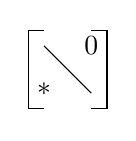
\begin{tikzpicture}
\node at (.2,.2) {*};
\node at (.8,.8) {0};
\draw[-] (.2,.8) to (.8,.2);
\draw[-] (0,0) to (0,1);
\draw[-] (0,0) to (.2,0);
\draw[-] (0,1) to (.2,1);
\draw[-] (1,0) to (1,1);
\draw[-] (.8,0) to (1,0);
\draw [-] (.8,1) to (1,1);
\end{tikzpicture}}} \pi 
\vcenter{\hbox{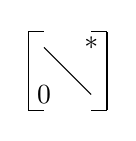
\begin{tikzpicture}
\node at (.2,.2) {0};
\node at (.8,.8) {*};
\draw[-] (.2,.8) to (.8,.2);
\draw[-] (0,0) to (0,1);
\draw[-] (0,0) to (.2,0);
\draw[-] (0,1) to (.2,1);
\draw[-] (1,0) to (1,1);
\draw[-] (.8,0) to (1,0);
\draw [-] (.8,1) to (1,1);
\end{tikzpicture}}}} = \overline{B_- \pi B_+} \subset \text{Mat}_n$$

For a linear representation $V$, the action $T \curvearrowright (V \supset X)$ gives us $[X \subset V] \in \text{Sym}T^{\ast} \simeq \Z[y_1, \dots, y_d]$.

Importantly, note that we can \textit{always} split $V$ as a direct sum of irreducible $T$-representations: \\
$$V \cong \bigoplus_{\text{weights }\lambda} \C_{\lambda}^{\oplus m_{\lambda}} \; \text{ for some multiplicities } m_{\lambda} \in \bN$$


Recall also our pipe dream formula, from yesterday's definition of the double Schubert polynomial $S_{\pi}$:
$$S_{\pi}(x_1, \dots, x_n, y_1, \dots, y_n) = [\overline{X_{\pi}} \subset \text{Mat}_n] = \sum_{\text{(pipe dreams for } \pi)} \prod_{\text{(crosses)}}x_{\text{row}} - y_{\text{col}}$$

\vspace{1em}

\begin{Definition}[Multigraded Hilbert series]
For a vector space $V$ of dimension $n$ (not necessarily equal to $\dim T)$, define $R \coloneqq \text{Fun}(V) \cong \C[z_1, \dots, z_n]$. Then the multigraded Hilbert series of $R$ is the formal sum
$$ h_R \coloneqq \sum_{\text{weights } \lambda \text{ of } T} \dim_{\C}(R_{\lambda})\, e^{\lambda}  \quad \in \mathbb{Z}[e^{\pm y_1}, \dots, e^{\pm y_d}]$$
where $R_{\lambda}$ is the $\lambda$-weight space of $R$.
\end{Definition}

Note that we have $h_{\oplus R_i} = \oplus h_{R_i}$.

To ensure the dimensions of the above weight spaces are finite, we impose the ``attractive condition" (we'll call it this, because we like it) that all $\lambda_i$ must lie in an open half-space.

\begin{Example}
We have the weight $\text{wt}(z_1^2 z_3) = -2 \lambda_1 - 1 \lambda_3$ (note that the coefficients are negative because we are acting on the dual space).
\end{Example}

\begin{Example}
For $n=1$, we have $\C[z_1] = \text{Fun}(V)$. So $h_R = \sum_{k=0}^{\infty} e^{-k \lambda_1} = \frac{1}{1-e^{-\lambda_1}}$.
\end{Example}

\begin{Example}
For general $n$, using the calculation directly above, we obtain $\C[z_1, \dots, z_n] \cong \C[z_1] \otimes \dots \otimes \C[z_n]$. So $h_R = \Pi_{i=1}^{n}  \frac{1}{1-e^{-\lambda_i}}$.
\end{Example}

\begin{Definition}[Multigraded / $T$-equivariant module]
If $R \curvearrowright M$, we say that $M$ is a multigraded (i.e. $T$-equivariant) module if:
\begin{itemize}
    \item $T \curvearrowright M$ (i.e. $M = \oplus_{\lambda \in T^{\ast}} M_{\lambda}$)
    \item $r \in R_{\lambda}, m \in M_{\mu} \implies rm \in M_{\lambda + \mu}$
\end{itemize} \end{Definition}

\begin{Definition}[Multigraded Hilbert series of an $R$-module $M$]
For $M$ a finitely generated $R$-module, we define 
$$ h_M \coloneqq \sum_{\text{weights } \lambda \text{ of } T} \dim(M_{\lambda}) \, e^{\lambda} $$
\end{Definition} 

Note from the definition above that the multigraded Hilbert series is so named because it is not graded by $\mathbb{Z}$ or $\mathbb{N}$, but by the weight lattice for $T$. Being multigraded is the same as having a torus action.

\begin{Example}
If $M = Rm$ (a free $R$-module with one generator), and $\text{wt}(m) = \lambda_m$, then $h_M = e^{\lambda_m} h_R$.
\end{Example}

A key example is the case $M = R/I$,  where $I$ is a $T$-invariant ideal, and $X = V(I)$. This motivates the next definition: notice that if $I=0$ (so $X$ is the entire space $V$), then we'd like $[V \subset V]$ to be 1. Directly above, though, we've already computed this to be a sum not equal to 1. The ``$K$-theoretical version" here will fix this issue.

\begin{Definition}
Letting $X = V(I)$, we have $[X \subset V]_K \coloneqq \frac{h_{R/I}}{h_R}$.
\end{Definition}

\begin{Theorem}
$[X \subset V]_K$ is a Laurent polynomial in $\{e^{\lambda}\}$.
\end{Theorem}
\begin{proof}
Sketch: If $R/I$ is a finitely generated module over a Noetherian ring $R$, and $I = (f_1, \dots, f_n)$, then there is a finite free resolution of $R/I$:
$$ 0 \to \dots \to \oplus_i R[\mu_i] \to R \to R/I \to 0 $$
So, this free resolution terminates, and the Hilbert series we want is an alternating sum of Hilbert series corresponding to the terms in the free resolution. Using that the series ``commutes with direct sum," and the fact that we've already computed series for single terms, we obtain a finite Laurent polynomial.
\end{proof}

\begin{Example}
If $X \subset V$ is a linear subspace, with $V = X \oplus X'$, then $[X \subset V]_K = \prod_{\mu \in X'}(1-e^{-\mu}) \in \Z[e^{\pm \mu}]$, whereas $[X \subset V] = \prod_{\mu \in X'} \mu \in \text{Sym}T^{\ast} = \Z[y_1, \dots, y_n]$.
\end{Example}

\noindent Next, let's check which axioms for $[X \subset V]$ are still satisfied by $[X \subset V]_K$:
\begin{enumerate}
    \item[\checkmark (0)] $[\{0\} \subset \{0\}]_K = 1$
    \item [\checkmark (2)] For a hyperplane $W = \{f=0\}$ with $X \subset W \subset V$, $[X \subset V]_K \coloneqq \frac{h_X}{h_V} = \frac{h_X}{h_W} \frac{h_W}{h_V} = [X \subset W]_K [W \subset V]_K$.
    \item[\checkmark (1)] With the setup above, and $X \subset V$, $X \not \subset W$, and $X$ reduced and irreducible, recall that $X = V(I)$ for $I$ a prime ideal $\iff$ $R/I$ is an integral domain.
    
    Letting $h_{X \cap W} \coloneqq h_{R/(I+(f))}$, we have exact sequence
    $$ 0 \to (R/I)f \hookrightarrow R/I \twoheadrightarrow R/(I + (f)) \to 0 $$
    This gives us an injection
    $$ 0 \to R/I \stackrel{\cdot f}{\to} (R/I)f \to 0 $$
    The second map $\cdot f$ above is an isomorphism of $R$-modules, but not in the multigraded sense. To fix this, we must introduce a shift by the weight $[e^{\wt(f)}]$, with $\wt(f) = -\wt(V(f)/W)$.
    Then, we indeed have $[X \subset V]_K = [X \cap W \subset W]_K$, and the axiom holds.
    
    \item[$\bigtimes$ \, (3)] This axiom no longer holds for $[X \subset V]_K$. For example, consider $R = \C[x,y]$, and $I = (x^2 - y^2)$. This is not a prime ideal; we can form quotients by $(x-y)$ or $(x+y)$, obtaining the following short exact sequence of    homogeneous graded $R$-modules:
    $$ 0 \to R/(x^2-y^2) \to R/(x-y) \oplus R/(x+y) \to R/(x,y) \to 0 $$
\centerline{\includegraphics[width=4in]{5.1.jpeg}}

\end{enumerate}
\vspace{1em}
\textbf{Question:} How do we relate $[X \subset V]$ and $[X \subset V]_K$?
\begin{Theorem}
Replace $\lambda$ by $\epsilon \lambda$, and take the leading term. That is:
$$ \lim_{\epsilon \to 0} \left( \frac{[X \subset V]_K}{\epsilon^{\text{codim}_v X}} \right) = [X \subset V] $$
\end{Theorem}

A last definition, which will soon be relevant:

\begin{Definition}[Subword complex]
If $Q$ is a word in the generators of a Coxeter group $W$, with $w \in W$, the subword complex $\Delta(Q,w)$ is a simplicial complex with vertices corresponding to the elements of $Q$.

A subword $F \subset Q$ is called a facet (i.e. a maximal face) precisely when $Q \setminus F$ is a reduced word for $w$.
\end{Definition}

\begin{Example}
Let $r_1$ be the transposition $(12) \in S_n$. Then $\Delta(121, r_1)$ (where $121$ is shorthand for $r_1 r_2 r_1$) is the simplicial complex pictured: \vspace{1em}

\centerline{\includegraphics[width=2in]{5.2.jpeg}}

Note that we index faces and vertices according to ``missing" letters in $Q$, and the complex above is homotopy equivalent to a point. Note also that the unpictured bottom edge, $-2-$ (i.e., $(23)$ in cycle notation), is \textit{not} a facet, because $r_2 = (23)$ is not a reduced word for $r_1$, whereas the other edges yield.
\end{Example}

\section{Lecture 6 (Allen Knutson)}
This lecture is split into two parts.  The first is a continuation of the previous lecture, leading up to an equivariant $K$-theory version of the AJS/Billey formula.  The second is a discussion of $G$-equivariant cohomology from the ground up.

\subsection{The subword complex and equivariant $K$-theory} Recall that given a word $Q$ in the primitive generators of a Coxeter group $W$, and some element $w\in W$, we can build the subword complex $\Delta(Q,w)$. The following theorem gives us a sense of what these look like:

\begin{Theorem}[Knutson-Miller '05] Let $\ell(w)$ denote the length of $w$. Then:
\begin{enumerate}
    \item $\dim \Delta(Q,w) = \# Q - \ell(w) - 1$.
    \item $\Delta (Q,w)$ is always homeomorphic to a ball or a sphere. It is also a $\Delta(Q,w)$ is a \textbf{shellable}  simplicial complex.  
    \item $\partial \Delta(Q,w) = \bigcup_{ w' > w} \Delta(Q,w')$.
\end{enumerate}
\end{Theorem}

We'll mention one other result that tells us something about the combinatorics of these complexes, namely about the links to their faces.

\begin{Example}
First, what's the link of a stratum in a stratified space?  Well, it's the intersection of the boundary of a small open neighborhood of that stratum.  Here's a picture of a link (red) of a stratum (blue), together with the ``combinatorialized'' version of the link available to a simplicial set:
\begin{center}
\includegraphics[width=4in]{6.1.png}
\end{center}
\end{Example}

The result will be stated using the following terminology:
\begin{Definition}
The \textbf{Mobius function} on the faces $F$ of a simplicial complex is
\[ \mu(F) := 1 - \chi(\textup{link of }F)\]
\end{Definition}

\begin{Theorem}
If $\Delta$ is a shellable ball or sphere, then 
    \[ \textup{link}(F) \cong \begin{cases} \textup{hemisphere} & \textup{for $F$ an exterior face}\\
    \textup{sphere} \cong S^{\textup{codim}{F} - 1} & \textup{for $F$ an interior face}\end{cases}\]
Translated, this gives:
\[\mu(F) = \begin{cases} 0 & \textup{for $F$ an exterior face}\\
   (-1)^{\text{codim}(F)}  & \textup{for $F$ an interior face}\end{cases}\]
In our case, where $\Delta = \Delta(Q,w)$, and is thus a shellable ball or sphere, this result implies that $\mu(F) = \pm1$ if $Q \setminus F$ doesn't contain a reduced word $w' \subset w$, and is 0 otherwise.
\end{Theorem}


OK, back to Schubert stuff, where we'll use some of the above terminology. Recall that given $v\in W$ and a reduced word $Q$ for $v$, AJS/Billey gives us a formula

\[ [ X_0^v \cap X_w] = \sum_{\textup{reduced subexpression }R\subseteq Q\\ = \textup{facets of $\Delta(Q,v)$}} stuff \quad \in H_T^*(X_0^v)\]

This is a statement in equivariant cohomology. We will see that there is also an analogous formula in equivariant $K$-theory!  To get there, the above language of the subword complex will be useful, in light of the following result:

\begin{Theorem}[Knutson] There exists a $T$-equivariant degeneration of the Kazhdan-Lusztig variety $X_0^v \cap X_w$ to the Stanley-Reisner variety of the subword complex:
\[ SR(\Delta(Q,w)) := \bigcup_{\textup{facets $F$ of }\Delta(Q,w)} \mathbb{C}^F \quad \subseteq \mathbb{C}^Q\]
\end{Theorem}

The fact that the degeneration is $T$-equivariant means that it drags along equivariant cohomology and $K$-theory classes. So in particular, this result implies the following promised $K$-theory version of AJS/Billey:
\begin{Theorem}[Graham-Willems]
Given $v\in W$ and a reduced word $Q$ for $v$,
\[ [ X_0^v \cap X_w]_K = \sum_{\textup{interior facets of $\Delta(Q,v)$}} (-1)^{|R|-\ell(w)}\Big(\prod_{q\in Q}r_q\cdot  \widehat{(1-e^{-\alpha_q})}\Big)\cdot 1 \quad \in K_T(X_0^v)\]
where the sum is now over subwords $R\subseteq Q$ such that $R$ contains a reduced word for $w$, but not for any $w' > w$; the notation $\widehat{(1-e^{-\alpha_q})}$ means that we only include this expression in the product if $q\in R$. 
\end{Theorem}

The above was about an $T$-equivariant $K$-theory class of an intersection inside the flag variety. Next, we'll have a formula for the $T\times T$-equivariant $K$-theory class of a matrix Schubert variety. Let's first give this a cool name:

\begin{Definition}
The \textbf{double Grothendieck polynomial} is 
\[ G_\pi(e^x, e^y) := [ \overline{X_\pi}]_K \in K_{T\times T}(\textup{Mat}_n) \cong K_{T\times T}(\textup{point}) = \mathbb{Z}[e^{\pm x_1}, \dots, e^{\pm x_n}, e^{\pm y_1}, \dots, e^{\pm y_n}]\]
\end{Definition}

\noindent It turns out that this also has a formula:

\begin{Theorem}[Fomin-Kirillov]
The double Grothendieck polynomial can be calculated as
\[G_\pi(e^x,e^y) = \sum_{\textup{possibly nonreduced pipe dreams for $\pi$}} (-1)^{\# \textup{extra $+$'s}} \prod_{+\textup{'s}} (1-e^{-x_{row} + y_{col}})\]
\end{Theorem}

\begin{Example}
For $\pi = 132$, recall from Lecture 1 that there are two reduced pipe dreams: 

\begin{center}
$\vcenter{\hbox{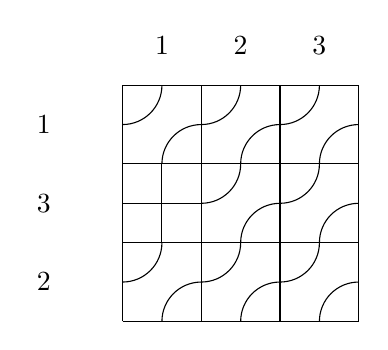
\begin{tikzpicture}
\draw[-] (1,4) to (4,4);
\draw[-] (4,4) to (4,1);
\draw[-] (4,1) to (1,1);
\draw[-] (1,1) to (1,4);
\node (1) at (1.5,4.5) {$1$};
\node (2) at (2.5,4.5) {$2$};
\node (3) at (3.5,4.5) {$3$};
\node (p1) at (0,3.5) {$1$};
\node (p2) at (0,2.5) {$3$};
\node (p3) at (0,1.5) {$2$};
\draw[-] (2,4) to (2,1);
\draw[-] (3,4) to (3,1);
\draw[-] (4,4) to (4,1);
\draw[-] (1,1) to (4,1);
\draw[-] (1,2) to (4,2);
\draw[-] (1,3) to (4,3);
\draw[-] (1,4) to (4,4);
\draw (1,3.5) arc[start angle=-90, end angle=0, radius=.5]; %11
\draw (1.5,3) arc[start angle=180, end angle=90, radius=.5]; 
\draw (2,3.5) arc[start angle=-90, end angle=0, radius=.5]; %12
\draw (2.5,3) arc[start angle=180, end angle=90, radius=.5];
\draw (3,3.5) arc[start angle=-90, end angle=0, radius=.5]; %13
\draw (3.5,3) arc[start angle=180, end angle=90, radius=.5];
\draw[-] (1,2.5) to (2,2.5); %21
\draw[-] (1.5,3) to (1.5,2);
\draw (2,2.5) arc[start angle=-90, end angle=0, radius=.5]; %22
\draw (2.5,2) arc[start angle=180, end angle=90, radius=.5];
\draw (3,2.5) arc[start angle=-90, end angle=0, radius=.5]; %23
\draw (3.5,2) arc[start angle=180, end angle=90, radius=.5];
\draw (1,1.5) arc[start angle=-90, end angle=0, radius=.5]; %31
\draw (1.5,1) arc[start angle=180, end angle=90, radius=.5];
\draw (3,1.5) arc[start angle=-90, end angle=0, radius=.5]; %32
\draw (2.5,1) arc[start angle=180, end angle=90, radius=.5];
\draw (2,1.5) arc[start angle=-90, end angle=0, radius=.5]; %33
\draw (3.5,1) arc[start angle=180, end angle=90, radius=.5];
\end{tikzpicture}}}$
\hspace{10mm} and \hspace{10mm}
$\vcenter{\hbox{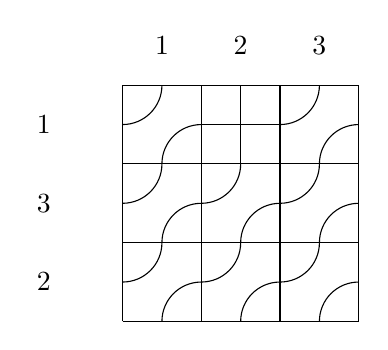
\begin{tikzpicture}
\draw[-] (1,4) to (4,4);
\draw[-] (4,4) to (4,1);
\draw[-] (4,1) to (1,1);
\draw[-] (1,1) to (1,4);
\node (1) at (1.5,4.5) {$1$};
\node (2) at (2.5,4.5) {$2$};
\node (3) at (3.5,4.5) {$3$};
\node (p1) at (0,3.5) {$1$};
\node (p2) at (0,2.5) {$3$};
\node (p3) at (0,1.5) {$2$};
\draw[-] (2,4) to (2,1);
\draw[-] (3,4) to (3,1);
\draw[-] (4,4) to (4,1);
\draw[-] (1,1) to (4,1);
\draw[-] (1,2) to (4,2);
\draw[-] (1,3) to (4,3);
\draw[-] (1,4) to (4,4);
\draw (1,3.5) arc[start angle=-90, end angle=0, radius=.5]; %11
\draw (1.5,3) arc[start angle=180, end angle=90, radius=.5]; 
\draw[-] (2.5,4) to (2.5,3); %12
\draw[-] (2,3.5) to (3,3.5);
\draw (3,3.5) arc[start angle=-90, end angle=0, radius=.5]; %13
\draw (3.5,3) arc[start angle=180, end angle=90, radius=.5];
\draw (1,2.5) arc[start angle=-90, end angle=0, radius=.5]; %21
\draw (1.5,2) arc[start angle=180, end angle=90, radius=.5];
\draw (2,2.5) arc[start angle=-90, end angle=0, radius=.5]; %22
\draw (2.5,2) arc[start angle=180, end angle=90, radius=.5];
\draw (3,2.5) arc[start angle=-90, end angle=0, radius=.5]; %23
\draw (3.5,2) arc[start angle=180, end angle=90, radius=.5];
\draw (1,1.5) arc[start angle=-90, end angle=0, radius=.5]; %31
\draw (1.5,1) arc[start angle=180, end angle=90, radius=.5];
\draw (3,1.5) arc[start angle=-90, end angle=0, radius=.5]; %32
\draw (2.5,1) arc[start angle=180, end angle=90, radius=.5];
\draw (2,1.5) arc[start angle=-90, end angle=0, radius=.5]; %33
\draw (3.5,1) arc[start angle=180, end angle=90, radius=.5];
\end{tikzpicture}}}$
\end{center}
\vspace{5mm}

There is also one (properly) nonreduced pipe dream, with two crossings, which is resolved by the above reduced two:

\begin{center}
    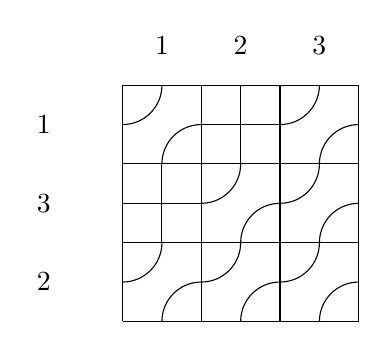
\begin{tikzpicture}
\draw[-] (1,4) to (4,4);
\draw[-] (4,4) to (4,1);
\draw[-] (4,1) to (1,1);
\draw[-] (1,1) to (1,4);
\node (1) at (1.5,4.5) {$1$};
\node (2) at (2.5,4.5) {$2$};
\node (3) at (3.5,4.5) {$3$};
\node (p1) at (0,3.5) {$1$};
\node (p2) at (0,2.5) {$3$};
\node (p3) at (0,1.5) {$2$};
\draw[-] (2,4) to (2,1);
\draw[-] (3,4) to (3,1);
\draw[-] (4,4) to (4,1);
\draw[-] (1,1) to (4,1);
\draw[-] (1,2) to (4,2);
\draw[-] (1,3) to (4,3);
\draw[-] (1,4) to (4,4);
\draw (1,3.5) arc[start angle=-90, end angle=0, radius=.5]; %11
\draw (1.5,3) arc[start angle=180, end angle=90, radius=.5]; 
\draw[-] (2.5,4) to (2.5,3); %12
\draw[-] (2,3.5) to (3,3.5);
\draw (3,3.5) arc[start angle=-90, end angle=0, radius=.5]; %13
\draw (3.5,3) arc[start angle=180, end angle=90, radius=.5];
\draw[-] (1,2.5) to (2,2.5); %21
\draw[-] (1.5,3) to (1.5,2);
\draw (2,2.5) arc[start angle=-90, end angle=0, radius=.5]; %22
\draw (2.5,2) arc[start angle=180, end angle=90, radius=.5];
\draw (3,2.5) arc[start angle=-90, end angle=0, radius=.5]; %23
\draw (3.5,2) arc[start angle=180, end angle=90, radius=.5];
\draw (1,1.5) arc[start angle=-90, end angle=0, radius=.5]; %31
\draw (1.5,1) arc[start angle=180, end angle=90, radius=.5];
\draw (3,1.5) arc[start angle=-90, end angle=0, radius=.5]; %32
\draw (2.5,1) arc[start angle=180, end angle=90, radius=.5];
\draw (2,1.5) arc[start angle=-90, end angle=0, radius=.5]; %33
\draw (3.5,1) arc[start angle=180, end angle=90, radius=.5];
\end{tikzpicture}
\end{center}

Therefore, by the Fomin-Kirillov formula, the double Grothendieck polynomial in this case is
\[ G_{132}(e^x, e^y) = (1-e^{-x_2 + y_1}) + (1-e^{-x_1 + y_2}) - (1-e^{-x_2 + y_1})(1-e^{-x_1 + y_2})\]
\end{Example}



\subsection{$G$-equivariant cohomology: what is it, really?}
Okay, changing gears! We've already seen some $G$-equivariant cohomology (and even some $G$-equivariant $K$-theory), but let's dive into the details a bit.

We all love integral cohomology. It's our favorite (contravariant) functor 
\[H^*: \frac{\{\textup{spaces, continuous maps}\}}{\textup{homotopy}} \to \textup{Rings}\]
Fixing a group $G$, we might wish to build a version of $H^*$, which we'll denote $H^*_G$, that goes like:
\[H_G^*: \frac{\{\textup{$G$-spaces, continuous $G$-equivariant maps}\}}{\textup{$G$-equivariant homotopy}} \to \textup{Rings}\]
In other words, we're shopping for some kind of topological invariant of $G$-spaces that is sensitive to the action itself (even though, confusingly, the action is not reflected in the notation ``$H_G^*$'' that we've chosen). Let's demand a few properties from $H_G^*$:
\begin{enumerate}
    \item if the $G$-action on $X$ is free, then $H_G^*(X) \cong H^*(X/G)$;
    \item if the $G$-space $C$ is contractible (but not necessarily $G$-equivariantly contractible), then $H_G^*(X \times C) \cong H_G^*(X)$, where the $G$-action on the product is the diagonal one.
\end{enumerate}
These are in fact a complete list of axioms of the theory.  Indeed, if $EG$ denotes any contractible space on which $G$ acts freely, then by (1) and (2) we have 
\[ H_G^*(X) \cong H_G^*(X\times EG) \cong H^*( (X\times EG)/G).\]
So we can calculate the equivariant cohomology of any $G$-space as the \textit{usual} cohomology of the \textbf{Borel mixing space} $(X\times EG)/G$ of the action. This space looks like an $X$-bundle over $EG/G =: BG$. 

To make use of this new invariant, we'll first need to build some $EG$'s. Let's do a few:

\begin{Example}
If $G=\Z$, we can take $E\Z := \mathbb{R}$ with the translation action. So $B\Z = S^1$.
\end{Example}

\begin{Example}
This will be the most important example for us. If $G=\mathbb{C}^\times$, we can take $E\mathbb{C}^\times := \mathbb{C}^\infty \setminus \{0\}$ with the diagonal action.  This space is contractible by a theorem in topology. By taking products, we get that we can take $E(\mathbb{C}^\times)^d := (E\mathbb{C}^\times)^d$. Another thing: since $B\mathbb{C}^\times \cong \mathbb{C}P^\infty$, we see that even the equivariant cohomology of a point can be huge: $H_{\mathbb{C}^\times}^*(\textup{point}) = H^*(\mathbb{C}P^\infty) = \mathbb{Z}[u], |u|=2$.
\end{Example}


\begin{Example}
If $G=GL_n\mathbb{C}$, we can take
\[ EGL_n\mathbb{C} := \{ n \times \mathbb{N} \textup{ matrices of rank $n$}\}\]
Repeatedly extracting the bottom row realizes $EGL_n\mathbb{C}$ as an iterated $(\mathbb{C}^\infty \setminus \{0\})$-bundle over $\mathbb{C}^\infty \setminus \{0\}$, and therefore it is contractible.

It's not so important that we know this example.  But since we do now, we can get a bunch of $EG$'s for free from the following simple observation: if $G\leq H$ is a subgroup, then $EH$ can serve as an $EG$!  So if $G \leq GL_n\mathbb{C}$ is any matrix group, we can just steal $EGL_n\mathbb{C}=:EG$.
\end{Example}

\begin{Remark}
If $G\leq H$ is a homotopy equivalence, then $H^*_G = H^*_H$. We will use this for a torus $T$ inside the Borels $B,B_-$.
\end{Remark}

\begin{Remark}
If $Y \subset X$ is a nice $G$-stable subset, then hopefully it's believable that it defines a class $[Y]_G \in H^*_G(X)$. We'll drop the subscript $G$ when it should be clear that something lives in equivariant cohomology. For example, both $[X_w^\circ]$ and $[X_w]$ refer to honest classes in $H_{B_-}^*(GL_n/B)$.
\end{Remark}

We'll calculate more with this later, but for now we'll take the $GL_n\mathbb{C}$-equivariant inclusion \fbox{$j: GL_n\mathbb{C} \hookrightarrow \textup{Mat}_n\mathbb{C}\simeq \textup{point}$} and extract a diagram that relates the classes we've encountered so far:

\begin{center}
\begin{tikzcd}
& & & \mathbb{Z}[x_1, \dots, x_n, y_1, \dots, y_n]\arrow[d,equals]\\
H^*_{B_-}(GL_n/B) & H^*_{B_-\times B}(GL_n)\arrow[l,equals] & H^*_{B_-\times
B}(\textup{Mat}_n\mathbb{C})\arrow[l,"j^*"'] \arrow[r,equals] & \overbrace{H^*_{T\times T}(\textup{point})}\\
\left[X_\pi\right] & \left[\overline{B_- \pi B}\right]\arrow[l,equals] & \left[\overline{\overline{B_- \pi B}}=: \overline{X_\pi}\right]\arrow[l,mapsto] & S_\pi (x,y)\arrow[l,equals]
\end{tikzcd}
\end{center}

Here is one more diagram that we can draw: for $v\in S_n$, there is the sequence of $T$-equivariant inclusions \fbox{$i_v: vB/B \hookrightarrow X_0^v \hookrightarrow GL_n/B$}, which gives

\begin{center}
    \begin{tikzcd}
    H_T^*(\textup{point}) \cong \mathbb{Z}[y_1, \dots, y_n]\arrow[d,equals] & & \\
    \overbrace{H^*_T(vB/B)} & H^*_T(X_0^v)\arrow[l,"i_v^*"'] & H_{T\simeq B_-}(GL_n/B)\arrow[l,"i_{X_0^v}^*"']\\
    \left[X_w\cap X_0^v\right]\big|_v \arrow[d,equals] & \left[X_w\cap X_0^v\right]\arrow[l,mapsto] & \left[X_w\right]\arrow[l,mapsto]\arrow[d,equals]\\
    S_w(x,y)|_{x_i := y_{v(i)}} & & S_w(x,y)
    \end{tikzcd}
\end{center}
This is a factorization of the map that just restricts to the $T$-fixed point $vB/B \in GL_n/B$.

\section{Lecture 7 (Paul Zinn-Justin)}

\section{Lecture 8 (Paul Zinn-Justin)}

\section{Lecture 9 (Allen Knutson)}

\section{Lecture 10 (Allen Knutson)}

\section{Lecture 11 (Paul Zinn-Justin)}

\section{Lecture 12 (Paul Zinn-Justin)}

\section{Lecture 13 (Allen Knutson)}

\section{Lecture 14 (Paul Zinn-Justin)}

\subsection{Basic Definitions}

\begin{Definition}[Temperley-Lieb Algebra]
	Let $\tau$ be a complex number. The \textbf{Temperley-Lieb algebra} $\TeL_n(\tau)$ is generated by an identity $1$ and generators $e_1, \ldots e_{n-1}$ satisfying the relations
	\begin{itemize}
		\item $e_i^2 = \tau e_i$
		\item $e_i e_{i+1} e_i = e_i$
		\item $e_i e_j = e_j e_i, |i-j|>1$
	\end{itemize}
\end{Definition}

We can give a pictorial description of this algebra: we regard each generator $e_i$ as corresponding to a diagram
\ctikzfig{TLfig1}
and regard $\tau$ as corresponding to the ``fugacity of a bubble." We then multiply by composing vertically (with the rightmost element at the top), and ``popping" bubbles to obtain a factor of $\tau$:
\ctikzfig{TLfig2}

\begin{Example}[$\TeL_3(\tau)$]
	When $n=3$, we have generators $1 = $ \tikzfig{TL3gen1}, $e_1 = $ \tikzfig{TL3gene1}, and $e_2 = $ \tikzfig{TL3gene2}. We also obtain
	\[e_1 e_2 = \tikzfig{TL3e1e2}\]
	and 
	\[e_2 e_1 = \tikzfig{TL3e2e1},\]
	so that $\TeL_3(\tau)$ is $5$-dimensional.
\end{Example}



\begin{Proposition}
	The dimension of $\TeL_n$ is
	\[\dim \TeL_n = C_n = \frac{(2n)!}{n!(n+1)!},\]
	the $n$th Catalan number.
\end{Proposition}

\subsection{Temperley-Lieb Algebras and the Yang-Baxter Equation} We can reinterpret the Yang-Baxter equation through the lens of Temperley-Lieb algebras. Let $\tau = -(q+q^{-1}), a(u) = qu-q^{-1}u^{-1},$ and $b(u) = u-u^{-1}.$ We can then regard $\Rcheck_i$ as an element of the algebra obtained by adding $u^\pm$ and $v^\pm$ to $\TeL_n(\tau)$:
\[\Rcheck_i(u) = a(u) 1 + b(u) e_i \in \TeL_n(\tau)[u^{\pm}, v^{\pm}].\]
One can check that the equation
\[\Rcheck_i(u) \Rcheck_{i+1}(uv) \Rcheck_i(v) = \Rcheck_{i+1}(v) \Rcheck_{i}(uv) \Rcheck_{i+1}(u)\]
holds; we may thus interpret the Yang-Baxter equation as an identity in $\TeL_n(\tau)[u^{\pm}, v^{\pm}].$

Via this identification, we can regard systems satisfying the Yang-Baxter equation as representations of this algebra $\TeL_n(-(q+q^{-1}))[u^{\pm}, v^{\pm}].$ We may obtain one such representation via the map 
\[\phi: \TeL_n(-(q+q^{-1})) \rightarrow \on{End}((\C^2)^{\otimes n})\]
sending
\[e_i \mapsto I \otimes I \otimes \ldots \otimes  I \otimes 
\begin{bmatrix}
	0 & 0 & 0 & 0\\
	0 & -q^{-1} & 1 & 0\\
	0 & 1 & -q & 0\\
	0 & 0 & 0 & 0
\end{bmatrix} \otimes I \otimes \ldots \otimes I,\]
where the matrix is located in the $i$ and $i+1$ coordinates. 

One can check that this map respects the Temperley-Lieb relations, and that it induces a representation $\rho: \TeL_n(-(q+q^{-1}))[u^{\pm}, v^{\pm}] \rightarrow \on{End}((\C^2)^{\otimes n})$ sending
\[\Rcheck_i(u) \mapsto I \otimes \ldots \otimes  I \otimes 
\begin{bmatrix}
	qu-q^{-1}u^{-1} & 0 & 0 & 0\\
	0 & u(q-q^{-1}) & u-u^{-1} & 0\\
	0 & u-u^{-1} & u^{-1}(q-q^{-1})& 0\\
	0 & 0 & 0 & qu-q^{-1}u^{-1}
\end{bmatrix} \otimes I \otimes \ldots \otimes I\]

\subsection{Loop Models}

\begin{Definition}[Loop Model]
	A \textbf{loop model} is an assignment of the tiles \tikzfig{LoopModelPiece1} and \tikzfig{LoopModelPiece2} to the $k \times n$ rectangle
	\ctikzfig{LoopModelRectangle}
\end{Definition}

We can compute the \textbf{fugacity} of a loop model with respect to a parameter $q \not = \pm 1$ by assigning a fugacity of $a(x_i/y_j)$ to the \tikzfig{LoopModelPiece1} tile, and $b(x_i/y_j)$ to the \tikzfig{LoopModelPiece2} tile, and multiplying by $\tau^{\#\text{ closed loops}}$, where $\tau = -(q+q^{-1})$. That is, the fugacity is
\[\tau^{\#\text{ closed loops}} \cdot \prod_{i=1}^{k}\prod_{j=1}^n
\begin{cases}
	a(x_i/y_j) & \tikzfig{LoopModelPiece1}\\
	b(x_i/y_j) & \tikzfig{LoopModelPiece2}
\end{cases}\]

When $q = \pm 1$, we instead assign weights of $a(x_i -y_j)$ and $b(x_i-y_j)$ respectively, so that the fugacity of the loop model is

\[\tau^{\#\text{ closed loops}} \cdot \prod_{i=1}^{k}\prod_{j=1}^n
\begin{cases}
	a(x_i - y_j) & \tikzfig{LoopModelPiece1}\\
	b(x_i - y_j) & \tikzfig{LoopModelPiece2}
\end{cases}\]

%Add a worked example of fugacity computation.

\subsection{Loop Models and Grassmannians}

Let $X = T^*\Gr(k, n)$ be the cotangent bundle of the Grassmannian. We wish to consider its $T \times \C^\times$-equivariant cohomology. Observe that
\[H_{T \times \C^\times}^*(X) \cong \Z[x_1, \ldots, x_k, y_1, \ldots, y_n, h]^{S_k}/\cI,\]
where:

\begin{itemize}
	\item The ring $\Z[x_1, \ldots, x_k, y_1, \ldots, y_n, h]^{S_k}$ consists of polynomials symmetric in the $x_i$, i.e., invariant under the action of $S_k$ on $x_1, \ldots, x_k$. \item $\cI$ is the ideal generated by polynomials which vanish when each $x_i$ is replaced by some (distinct) $y_j$. 
	%is this actually correct? I have in my notes that $\cI = \cap \ker \phi_I,$ but I'm not sure that agrees with the example PZJ gave for $k=1$.
	That is, for any $I \in \binom{[n]}{k}$, we can define a map 
	\[\phi_I: \Z[x_1, \ldots, x_k, y_1, \ldots, y_n, h]^{S_k} \rightarrow \Z[y_1, \ldots y_n, h]\] 
	which sends $p(x_1, x_2, \ldots, x_k, y_1, \ldots, y_n, h)$ to $p(y_{I_1}, y_{I_2}, \ldots, y_{I_k}, y_1, \ldots, y_n, h).$ Note that the order on the elements of $I$ does not matter, since $p$ is symmetric in the $x_i.$ Then $\cI$ is the ideal generated by the kernels of the $\phi_I.$
\end{itemize}
For example, when $k=1$, we have that $\cI = \langle (x_1 - y_1), (x_1-y_2), \ldots, (x_1-y_n) \rangle,$ so that
\[H_{T \times \C^\times}^*(\Gr(1,n)) \cong \Z[x_1, y_1, \ldots, y_n, h]^{S_k}/\cI\]

Now, for each $I \in \binom{[n]}{k}$, let $X_I^\circ = B_{-}\C^I,$ where $\C^I$ is the coordinate subspace spanned by $e_{I_1}, \ldots, e_{I_k},$ denote the Schubert cell corresponding to $I$. One can check that $X_I^\circ  \cong \C^{k(n-k)-\on{inv}(I)},$ where $\on{inv}(I)$ is the inversion number of the binary string corresponding to $I$. In particular, $X_I^\circ$ is smooth.

Let $C_I = \overline{\C_{X_I^\circ} \Gr(k, n)}$ denote the closure of the conormal bundle of $X_I^\circ$ in $T^*(\Gr(k,n)).$ Let $\Stil_I = [C_I] \in H_{T \times \C^\times}^*(X)$ be the fundamental class of this conormal bundle.

Recall that when examining $H_T^*(\Gr(\cdot, n)),$ the $T$-equivariant cohomology of $\bigsqcup_{k=1}^n \Gr(k,n),$ we assigned 
\[S_I \mapsto \bigotimes_{i=1}^n \begin{cases}
	\begin{pmatrix}
		1 & 0
	\end{pmatrix}^{Tr} & i \not \in I\\
	\begin{pmatrix}
		0 & 1
	\end{pmatrix}^{Tr} & i \in I
\end{cases}\]

In the case of the cotangent bundle, we attach an element of $(\C^2)^{\otimes n}$ to each $\Stil_I$ via \textbf{link patterns}. We begin with the binary string associated to $I$, and repeatedly attach links between each substring of $1 0$, ignoring previously linked letters. This is perhaps most easily illustrated with an example: if our binary string is $01101001$, the associated link pattern would be \ctikzfig{LinkPattern}
To the link \tikzfig{LinkPatternij} between positions $i$ and $j$, we associate
$\begin{pmatrix}
	1\\
	0
\end{pmatrix}_i
\otimes
\begin{pmatrix}
	0\\
	1
\end{pmatrix}_j
-
q^{-1}
\begin{pmatrix}
	0\\
	1
\end{pmatrix}_i
\otimes
\begin{pmatrix}
	1\\
	0
\end{pmatrix}_j,
$
while to a ``lonely" $0$ or $1$ in position $i$ we associate $\begin{pmatrix} 1\\ 0\end{pmatrix}_i$ and $\begin{pmatrix} 0\\ 1\end{pmatrix}_i$ respectively. We then take the tensor product over the vectors associated to all links/lonely elements. 

\begin{Theorem}[Z-J, \href{https://doi.org/10.3842/SIGMA.2018.069}{Loop Models and $K$-Theory}, 2016]
	$\Stil_I = [C_I]$ is equal to the loop model partition function on a $k \times n$ rectangle where the connectivity of the external points satisfy:
	\begin{itemize}
		\item No bottom points are connected to other bottom points
		\item No top points are connected to right points
		\item The top lines reproduce the link pattern of the associated binary string.
	\end{itemize}
\end{Theorem}

\section{Lecture 15 (Allen Knutson)}

\section{Lecture 16 (Allen Knutson)}

\section{Lecture 17 (Paul Zinn-Justin)}

\section{Lecture 18 (Paul Zinn-Justin)}

\end{document}
